% !TEX root = ../master-thesis.tex




% Pauli crystall \cite{holten_observation_2021}

% DPP: \cite{kulesza_determinantal_2012}, \cite{hough_determinantal_2006}

A central challenge in quantum many-body systems involving indistinguishable fermionic particles is the accurate modeling of the fermionic antisymmetry in the many-body wavefunction. Even in the case of non-interacting fermions, the generation of realistic samples of experimentally observable quantities—such as single-shot atomic density measurements—requires proper antisymmetrization. As the number of particles and the dimensionality of the system increase, enforcing these antisymmetric constraints becomes computationally demanding. For example, treating antisymmetric wavefunctions explicitly for as few as four fermions in two dimensions already presents nontrivial computational difficulties.

To mitigate this challenge, Determinantal Point Processes (DPPs) are employed as a probabilistic framework inherently suited to capturing fermionic statistics. DPPs naturally model repulsive correlations between particles, reflecting the Pauli exclusion principle, and provide a mathematically principled and computationally efficient approach for sampling particle configurations from single-particle wavefunctions.

In experiments reporting the observation of "Pauli crystals"—ordered spatial structures emerging solely from quantum statistical effects—analytical sampling expressions have been derived under restrictive symmetry assumptions. However, in broader experimental contexts, such analytical forms are typically unavailable. In these cases, the DPP-based approach offers a general-purpose numerical method for simulating atomic distributions across diverse trapping geometries.

The following sections present a formal mathematical description of Determinantal Point Processes, detail the algorithmic procedures for DPP sampling, and compare the computational efficiency with that of direct antisymmetrization. The method’s practical utility is illustrated through numerical examples, including the reproduction of characteristic correlation features (see Fig.\ref{fig:interference}) using DPP-based simulations (see Fig.\ref{fig:interference-dpp}).

\begin{figure}
    \centering
    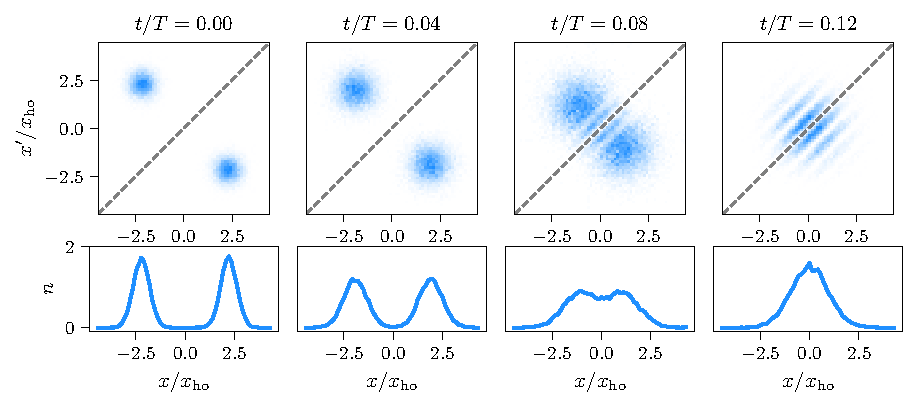
\includegraphics{fig-py/interference_dpp.pdf}
    \caption{DPP based}
    \label{fig:interference-dpp}
\end{figure}


\textbf{Mathematical formulation.}
Formally, a Determinantal Point Process on a space $\Lambda$ equipped with a suitable reference measure $\mu$ is defined through a kernel function $K(x,y)$, where $x,y \in \Lambda$. For a DPP, the probability of observing a configuration of points $\{x_1, x_2, \ldots, x_n\}$ is proportional to the determinant of a corresponding kernel matrix formed by evaluating $K$ at these points:
\begin{equation}
P(x_1, x_2, \ldots, x_n) \propto \det[K(x_i, x_j)]_{1 \leq i,j \leq n}.
\end{equation}
This determinantal structure naturally encodes repulsive correlations between points, making DPPs particularly well-suited for modeling fermionic systems where identical particles exhibit antisymmetric quantum statistics. Specifically, the kernel $K(x,y)$ typically corresponds to the two-point correlation function derived from the underlying single-particle wavefunctions:
\begin{equation}
K(x, y) = \sum_{k} \lambda_k \phi_k(x)\phi_k^*(y),
\end{equation}
where $\{\phi_k\}$ form an orthonormal set of eigenfunctions of a corresponding integral operator, and $\{\lambda_k\}$ are the associated eigenvalues, bounded between 0 and 1 to guarantee the existence of the process \cite{hough_determinantal_2006}.

The fundamental advantage of DPPs lies in their efficient sampling procedure, which bypasses the combinatorial complexity of directly antisymmetrizing wavefunctions. Specifically, if the kernel represents a projection operator (i.e., $\lambda_k$ equals either 0 or 1), the DPP simplifies to a projection DPP, significantly enhancing computational tractability.

% Sampling algorithm section

Given a projection kernel $K$, the sampling procedure of a projection DPP begins by computing the eigen-decomposition of the kernel $K$:
\begin{equation}
K(x,y) = \sum_{k=1}^{M} \phi_k(x)\phi_k^*(y),
\end{equation}
where $\{\phi_k\}$ form an orthonormal basis of the subspace associated with eigenvalue 1.
The algorithm then initializes an empty set $Y$ and proceeds iteratively. At each iteration, selection probabilities are computed proportional to:
\begin{equation}
p(x) = \frac{1}{M} \sum_{k=1}^{M} |\phi_k(x)|^2.
\end{equation}
A point $x$ is selected according to $p(x)$, after which the subspace is updated by projecting out the selected function:
\begin{equation}
\phi_k(x) \rightarrow \phi_k(x) - \sum_j \frac{\phi_j(x_{\text{selected}})}{\phi_j(x)} \phi_k(x_{\text{selected}}),
\end{equation}
and the resulting basis set is renormalized. The selected point is added to $Y$, $M$ is decreased, and the process repeats until $M = 0$. This approach efficiently generates sample realizations that adhere to the correct fermionic antisymmetry without explicitly antisymmetrizing wavefunctions.

% Computational complexity section
% \section*{\textbf{Computational complexity}}

Direct antisymmetrization of wavefunctions involves computing determinants of large matrices for every possible configuration, resulting in computational complexity that scales factorially with the particle number. In contrast, the projection-DPP sampling method described above significantly reduces complexity. It scales polynomially in both the number of points sampled and the number of eigenfunctions, typically providing practical feasibility for experimental scenarios involving tens or hundreds of particles.

Nevertheless, obtaining the eigen-decomposition of the kernel can become computationally intensive for large continuous spaces. Therefore, numerical implementations typically utilize efficient algorithms and GPU acceleration to handle realistic experimental scales, as demonstrated earlier in this thesis. The application of this DPP sampling approach was illustrated by replicating the quantum correlation results previously shown in Fig.~\ref{fig:interference}, demonstrating how realistic experimental snapshots can be efficiently generated using Determinantal Point Processes (Fig.~\ref{fig:interference-dpp}).
